\subsection{IASI Band 3 (2000-2760\invcm)}
%-----------------------------------------

\subsubsection{WVO results}
%..........................
% wvo plots
\begin{figure}[htp]
  \centering
  \includegraphics[scale=0.8]{graphics/iasiB3/iasiB3.wvo1_dtb_sfc.eps}
  \caption{IASI band 3 brightness temperature residuals for all view angles and profiles between using the true total transmittance profiles and those derived from the WVO1 set (see table \ref{tab:derived_set_combo})}
  \label{fig:iasiB3.wvo1_dtb_sfc}
  \vspace{1em}
  \includegraphics[scale=0.8]{graphics/iasiB3/iasiB3.wvo1_dtb.eps}
  \caption{IASI band 3 brightness temperature residual statistics between using the true total transmittance profiles and those derived from the WVO1 set (see table \ref{tab:derived_set_combo}). Compiled for all view angle and profile combinations. \textbf{(Top panel)} Average T\subscript{B} residuals. \textbf{(Middle panel)} RMS T\subscript{B} residuals. \textbf{(Bottom panel)} Maximum T\subscript{B} residuals.}
  \label{fig:iasiB3.wvo1_dtb}
\end{figure}

\begin{figure}[htp]
  \centering
  \includegraphics[scale=0.8]{graphics/iasiB3/iasiB3.wvo2_dtb_sfc.eps}
  \caption{IASI band 3 brightness temperature residuals for all view angles and profiles between using the true total transmittance profiles and those derived from the WVO2 set (see table \ref{tab:derived_set_combo})}
  \label{fig:iasiB3.wvo2_dtb_sfc}
  \vspace{1em}
  \includegraphics[scale=0.8]{graphics/iasiB3/iasiB3.wvo2_dtb.eps}
  \caption{IASI band 3 brightness temperature residual statistics between using the true total transmittance profiles and those derived from the WVO2 set (see table \ref{tab:derived_set_combo}). Compiled for all view angle and profile combinations. \textbf{(Top panel)} Average T\subscript{B} residuals. \textbf{(Middle panel)} RMS T\subscript{B} residuals. \textbf{(Bottom panel)} Maximum T\subscript{B} residuals.}
  \label{fig:iasiB3.wvo2_dtb}
\end{figure}

\subsubsection{DOZ results}
%..........................
% doz plots
\begin{figure}[htp]
  \centering
  \includegraphics[scale=0.8]{graphics/iasiB3/iasiB3.doz1_dtb_sfc.eps}
  \caption{IASI band 3 brightness temperature residuals for all view angles and profiles between using the true total transmittance profiles and those derived from the DOZ1 set (see table \ref{tab:derived_set_combo})}
  \label{fig:iasiB3.doz1_dtb_sfc}
  \vspace{1em}
  \includegraphics[scale=0.8]{graphics/iasiB3/iasiB3.doz1_dtb.eps}
  \caption{IASI band 3 brightness temperature residual statistics between using the true total transmittance profiles and those derived from the DOZ1 set (see table \ref{tab:derived_set_combo}). Compiled for all view angle and profile combinations. \textbf{(Top panel)} Average T\subscript{B} residuals. \textbf{(Middle panel)} RMS T\subscript{B} residuals. \textbf{(Bottom panel)} Maximum T\subscript{B} residuals.}
  \label{fig:iasiB3.doz1_dtb}
\end{figure}

\begin{figure}[htp]
  \centering
  \includegraphics[scale=0.8]{graphics/iasiB3/iasiB3.doz2_dtb_sfc.eps}
  \caption{IASI band 3 brightness temperature residuals for all view angles and profiles between using the true total transmittance profiles and those derived from the DOZ2 set (see table \ref{tab:derived_set_combo})}
  \label{fig:iasiB3.doz2_dtb_sfc}
  \vspace{1em}
  \includegraphics[scale=0.8]{graphics/iasiB3/iasiB3.doz2_dtb.eps}
  \caption{IASI band 3 brightness temperature residual statistics between using the true total transmittance profiles and those derived from the DOZ2 set (see table \ref{tab:derived_set_combo}). Compiled for all view angle and profile combinations. \textbf{(Top panel)} Average T\subscript{B} residuals. \textbf{(Middle panel)} RMS T\subscript{B} residuals. \textbf{(Bottom panel)} Maximum T\subscript{B} residuals.}
  \label{fig:iasiB3.doz2_dtb}
\end{figure}

\subsubsection{WVD results}
%..........................
% wvd plots
\begin{figure}[htp]
  \centering
  \includegraphics[scale=0.8]{graphics/iasiB3/iasiB3.wvd1_dtb_sfc.eps}
  \caption{IASI band 3 brightness temperature residuals for all view angles and profiles between using the true total transmittance profiles and those derived from the WVD1 set (see table \ref{tab:derived_set_combo})}
  \label{fig:iasiB3.wvd1_dtb_sfc}
  \vspace{1em}
  \includegraphics[scale=0.8]{graphics/iasiB3/iasiB3.wvd1_dtb.eps}
  \caption{IASI band 3 brightness temperature residual statistics between using the true total transmittance profiles and those derived from the WVD1 set (see table \ref{tab:derived_set_combo}). Compiled for all view angle and profile combinations. \textbf{(Top panel)} Average T\subscript{B} residuals. \textbf{(Middle panel)} RMS T\subscript{B} residuals. \textbf{(Bottom panel)} Maximum T\subscript{B} residuals.}
  \label{fig:iasiB3.wvd1_dtb}
\end{figure}

\begin{figure}[htp]
  \centering
  \includegraphics[scale=0.8]{graphics/iasiB3/iasiB3.wvd2_dtb_sfc.eps}
  \caption{IASI band 3 brightness temperature residuals for all view angles and profiles between using the true total transmittance profiles and those derived from the WVD2 set (see table \ref{tab:derived_set_combo})}
  \label{fig:iasiB3.wvd2_dtb_sfc}
  \vspace{1em}
  \includegraphics[scale=0.8]{graphics/iasiB3/iasiB3.wvd2_dtb.eps}
  \caption{IASI band 3 brightness temperature residual statistics between using the true total transmittance profiles and those derived from the WVD2 set (see table \ref{tab:derived_set_combo}). Compiled for all view angle and profile combinations. \textbf{(Top panel)} Average T\subscript{B} residuals. \textbf{(Middle panel)} RMS T\subscript{B} residuals. \textbf{(Bottom panel)} Maximum T\subscript{B} residuals.}
  \label{fig:iasiB3.wvd2_dtb}
\end{figure}
